% 2018 北京卷文第7题：单位圆上的四段候选弧（据固定源第1063页重绘）
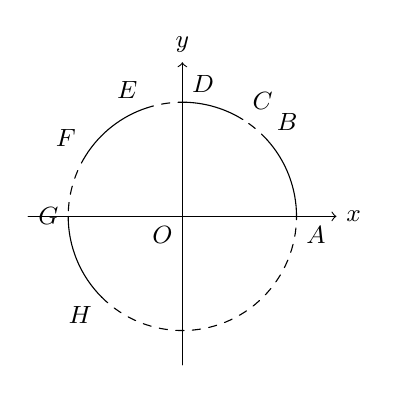
\begin{tikzpicture}[scale=1.45, font=\small, line cap=round]
  \draw[->] (-1.35,0)--(1.35,0) node[right] {$x$};
  \draw[->] (0,-1.3)--(0,1.35) node[above] {$y$};
  % 仅四段候选弧为实线；其余圆周分段画虚线
  \draw (1,0) arc (0:42:1);
  \draw[dashed] (42:1) arc (42:58:1);
  \draw (58:1) arc (58:88:1);
  \draw[dashed] (88:1) arc (88:108:1);
  \draw (108:1) arc (108:148:1);
  \draw[dashed] (148:1) arc (148:180:1);
  \draw (180:1) arc (180:225:1);
  \draw[dashed] (225:1) arc (225:360:1);
  \node[below left] at (0,0) {$O$};
  \node[below right] at (1,0) {$A$};
  \node[above right] at (42:1) {$B$};
  \node[above right] at (58:1) {$C$};
  \node[above right] at (0,1) {$D$};
  \node[above left] at (108:1) {$E$};
  \node[above left] at (148:1) {$F$};
  \node[left] at (180:1) {$G$};
  \node[below left] at (225:1) {$H$};
\end{tikzpicture}
